\documentclass[12pt]{article}
\usepackage{inputenc}
\usepackage[top=1in, bottom=1in, left=1in, right=1in]{geometry}
\usepackage{setspace}
\doublespacing
\usepackage{parskip}
\setcounter{secnumdepth}{1}
\pagestyle{myheadings}
\usepackage{graphicx}
%\usepackage{fontspec}
%\setmainfont{Georgia}
\setlength{\parindent}{1cm}
% These next three lines hide the citation keys in the bibliography, pretty cool.
%\makeatletter
%\def\@biblabel#1{}
%\makeatother
% These lines define the hanging indent! NEAT!
\makeatletter
% \renewcommand\@biblabel[1]{#1} % No brackets for the references
\def\@biblabel#1{}
\renewenvironment{thebibliography}[1]
     {\section*{\refname}%
      \@mkboth{\MakeUppercase\refname}{\MakeUppercase\refname}%
      \list{\@biblabel{\@arabic\c@enumiv}}%
           {\settowidth\labelwidth{\@biblabel{#1}}%
            \leftmargin\labelwidth
            \advance\leftmargin20pt% change 20 pt according to your needs
            \advance\leftmargin\labelsep
            \setlength\itemindent{-20pt}% change using the inverse of the length used before
            \@openbib@code
            \usecounter{enumiv}%
            \let\p@enumiv\@empty
            \renewcommand\theenumiv{\@arabic\c@enumiv}}%
      \sloppy
      \clubpenalty4000
      \@clubpenalty \clubpenalty
      \widowpenalty4000%
      \sfcode`\.\@m}
     {\def\@noitemerr
       {\@latex@warning{Empty `thebibliography' environment}}%
      \endlist}
\renewcommand\newblock{\hskip .11em\@plus.33em\@minus.07em}
\makeatother

\usepackage[compact]{titlesec}  
\titlespacing{\section}{0pt}{0pt}{0pt}


\begin{document}
% Manual Heading
{\raggedleft{}Gabriel Griggs} \\
Professor G. Felicitas Munzel \\
Seminar 5: PLS 43101 - 02 \\
Thursday, November 21st 2013\\
\centerline{Providence in the ``Life of Humanity'':}
\centerline{A Critical Analysis of Tolstoy's Calculus}
 
% \title{Providence in the ``Life of Humanity'': A Critical Analysis of Tolstoy's Calculus}
%\date{\vspace{-1in}} % this is a way to remove spaces without using the Titling package... 
% \author{Gabriel Griggs} % it sounds like this is supposed to be anonymous
% \maketitle
% \section{Introduction and Statement of Thesis}

Tolstoy's \emph{War and Peace} is both a novel and an argument on the proper interpretation and methodology of history. This argument is at odds with the literary form: the novel captures certain elements of life and daily existence that cannot be reduced to a mere philosophical argument. The novel, for example, is able to evoke strong emotions and empathy with the characters. In this dichotomy of forms, the tension between independence of personality, also known as free will, and the laws of history is palpable. This very dichotomy points to the difficulty of reducing human life, and consequently, human history to reason and the laws of nature. In other words, Tolstoy's argument of the second epilogue, that ``in the present case it is similarly necessary to renounce a freedom that does not exist, and to recognize a dependence of which we are not conscious,'' is not fully supported by the events of the novel itself.\footnote{Leo Tolstoy, \emph{War and Peace: The Maude Translation, Backgrounds and Sources, Criticism}, trans. Louise Maude and Aylmer, ed. George Gibian (New York: Norton, 1996, Print), 1074.}

Instead, what emerges from this tension between the novel and the philosophical argument of historical interpretation is a nuanced account of providence which is characterized by these aspects: (i) human beings have free will, but they can also fall into situations in which they lose this free will to a deterministic, machinistic force (such as the force that overcomes soldiers as they execute Platon Karataev); (ii) contrary to the arguments of the second epilogue, those who are in the proper state of mind are able to grow in inner freedom at precisely the time in which their external freedom is decreasing (Pierre as a prisoner and Andrew near his death); (iii) this state of mind, that allows for this inner freedom, is dependent on simple faith in God's providence --- faith that all is being shaped for a greater good despite not knowing \emph{how} it is being shaped.

% \section{Layout of the Paper}
We will begin by analyzing the tension of the primary literary forms: the narrative of the novel and the historical-philosophical argument for Tolstoy's interpretation of history. We will then continue to apply Tolsoy's new historical method which is essentially historical calculus. From this analysis, it should become clear that the novel is not resolved on giving up free will entirely in order to find historical laws. Instead, it affirms the presence of both historical, deterministic laws and the operation of free will. Thus, in order to resolve these two, there must be an operation of divine providence. Providence is the logical answer to this false dichotomy between free will and historical determinism as it allows for human free will, while at the same time allowing for history moving towards a particular purpose. This is not only a logical answer to the false dichotomy. Providence is fully fleshed out in the novel in the lives of Pierre, Andrew and Platon Karataev in particular. An analysis of these characters, through the lens of Tolstoy's historical calculus, reveals an explicit and coherent account of providence.

\section{Dichotomy of Forms: The Inherent Tension within \emph{War and Peace}} 
Tolstoy explicitly explains in his second epilogue that the conception of free will that institutions and churches depend on --- a conception that is implicit in conceptions of the soul and good and evil --- must necessarily be cast aside in order for the laws of inevitability to be found: ``Just so it now seems as if we have only to admit the law of inevitability, to destroy the conception of the soul, of good and evil, and all the institutions of state and church that have been built on up on those conceptions.''\footnote{Tolstoy, 1074.} Yet, especially coming in the second epilogue, this necessity of casting aside free will seems to be quite at odds with the novel that we have just read. In this novel, while there are certainly moments of inevitability, there are also certainly great moments of inner freedom and free will. In particular, there are areas in which free will manifests itself in beautiful and free human interactions.
 
If the laws of inevitability are true, how are we to explain the transformative experiences, the good and wholesome marriages found in the first epilogue and the unexplainable love of General Bolkonski for his daughter? Are these not presented in the novel as certain transcendent experiences of tenderness, joy and beauty? These transcendent experiences are all the more transcendent because they are manifestations of free will. Pierre did not have to marry Natasha, for example. He entered the marriage of his own accord, unlike his previous marriage to Helene. These are the very transcendent experiences, the ``life of nations and of humanity,'' that Tolstoy cannot fully capture with words. He himself admits that to ``seize and put into words, to describe directly the life of humanity or even of a single nation, appears impossible.''\footnote{Tolstoy, 1073.} And yet he still attempts to describe the ``life of humanity'' in his novel. We are left, then, in a situation in which the very dichotomy between free will and historical determinism seems to be pulling the author in two ways. This is represented in the false dichotomy of forms: novel and philosophical argument. This tension will ultimately be resolved with an account of providence.

\section{A New Historical Method: The Differential of \mbox{History}}
The best place to begin is Tolstoy's argument for a certain historical method through which the continuous ``movement of humanity, arising as it does from unnumerable arbitrary human wills'' is to be understood.\footnote{Tolstoy, 734.} In the beginning of Book XI, Tolstoy explains that Achilles is not able to catch the tortoise because he must always reach the point where the tortoise had been. But, by the time he has reached this point, the tortoise has already moved. This illustrates the limitations of discrete mathematical reasoning. We must employ the study of continuous motion to solve the paradox --- a study that is very similar to Newton's Calculus.

When we employ continuous thinking we realize that the error in the Achilles-tortoise paradox lies in the fact that Achilles' motion is faster than the tortoise's. In other words, Achilles' velocity function is not defined as ``catch up to the rabbit and stop'', as if it were operating in discrete and non-continuous units of time. Instead, his velocity is defined continuously over time. This being the case, there will be a point at which Achilles is at the same exact spot as the tortoise at the same exact time. In a position versus time graph, with position on the y-axis and time on the x-axis, we would see that the position-time curve of Achilles would eventually intersect with the position-time curve of the tortoise. After this point, because Achilles' velocity is always greater than the tortoise's velocity, his position will be ahead of the tortoise's position. An intuitive, continuous understanding of mathematics and physics enables us to resolve this paradox.

Similarly, Tolstoy argues, historical analysis must adopt a continuous method: ``Only by taking infinitesimally small units for observation (the differential of history, that is, the individual tendencies of men) and attaining to the art of integrating them (that is, finding the sum of these infinitesimals\footnote{A brief note on integration: imagine a curve on an xy-graph. The y-axis is the value of $f(x)$, a function that takes a value of $x$. A differential is represented as an infinitesimally small unit of $x$. By drawing out many of these differentials, we will eventually be able to piece together the shape of the original function which we were trying to approximate. Thus, in carrying on Tolstoy's analogy, by filling in enough differentials of history we should be able to calculate the exact function that created the outline of those differentials. For a further explanation, see the graph in the appendix.}) can we hope to arrive at the laws of history.''\footnote{Tolstoy, 732.} It is precisely this differential of history, the everyday actions of men, that is explored throughout the novel. Consequently, it follows that the novel is also the integral of these infinitesimals. One law of history that Tolstoy claims to have found through this method of history is the randomness and chaos of military victory, as well as the proportional relationship between the spirit of the army and the size of the army: ``The spirit of an army is the factor which multiplied by the mass gives the resulting force.''\footnote{Tolstoy, 914.} This is, unsurprisingly, a historical formulation of the first law of Newtonian physics, \emph{Force $=$ Mass $x$ Acceleration}, which coincided with Newton's development of calculus. It is this very spirit of the army that Kutuzov leverages in order to achieve military victory.

Despite these historical laws arising from Tolstoy's historical calculus, it is the differential of calculus that seems to transcend the laws of inevitability. Using Kutuzov as an example, we learn that by ``long years of military experience he knew, and with the wisdom of age understood, that it is impossible for one man to direct hundreds of thousands of others struggling with death, and he knew that the result of a battle is decided not by the orders of a commander in chief ... but by that intangible force called the spirit of the army, and he watched this force and guided it in as far as that was in his power.''\footnote{Tolstoy, 718.} Notice the simplicity and humility in Kutuzov's acknowledgment of a force greater than himself, while at the same time the acknowledgement of the narrator that Kutuzov is \emph{actually} affecting the battle by leveraging the spirit of the army. This implies that although there is a historical law at work, there is also an element of human free will at work at the same time.

This ability to operate with and leverage these deterministic laws of history lies in a unique characteristic of Kutuzov: his simplicity. Kutuzov does not trick himself into believing that he is a great man --- great in the eyes of the historians, as Napoleon is. Instead, Kutuzov is a very real model of humility. His humility enables him to be in touch with the spirit of the army and it also enables him to direct this force. This humility is one of the keys to operating within providence.

\section{Free Will, Humility and Absurdity: An Introduction to Providence}
There is a similar humility found in Mary: ``how can we, miserable sinners that we are, know the terrible and holy secrets of providence.''\footnote{Tolstoy, 80.} Mary is our first example of an explicit belief in providence, as opposed to a belief in laws of inevitability. Her view of providence is also opposed to the belief of the great military strategists who believe that they can control their own outcomes. Pierre will eventually come to believe in this same providence. This is seen in his assertion: ``To endure war is the most difficult subordination of man's freedom to the law of God... Simplicity is submission to the will of God; you cannot escape from Him.''\footnote{Tolstoy, 750.} Simplicity is present in the everyday interactions, in the differential of history. As seen in Pierre's words, simplicity is connected to belief in providence. It is fitting, then, that Christ is the key to this simplicity, as the narrator explicitly tells us: ``For us with the standard of good and evil given us by Christ, no human actions are incommensurable. And there is no greatness where simplicity, goodness, and truth are absent.''\footnote{Tolstoy, 946.} Christ is also the key to understanding providence's relationship with free will in that his death is a prime example of a human being freely submitting to the will of God.

If these laws of inevitability do indeed threaten to ``destroy the conception of the soul, of good and evil,''\footnote{Tolstoy, 1074.} how are we to resolve this dilemma? An answer comes in a close analysis of the analogy to astronomy: ``So also in history the new view says: 'It is true that we are not conscious of our dependence, but by admitting our free will we arrive at absurdity, while by admitting our dependence on the external world, on time, and on cause, we arrive at laws.'\thinspace''\footnote{Tolstoy, 1074.} The trouble here is that the historian, like a physicist, is seeking certainty and discounting the possibility of \emph{absurdity that is the manifestation of free will intersecting with providence.} 

In other words, the narrator is arguing that the historian must ignore absurdity as simply something that we cannot yet account for with the laws of inevitability: ``Free will is for history only an expression for the unknown remainder of what we know about the laws of human life.''\footnote{Tolstoy, 1072.} But to ignore the absurdity of the `life of humanity' is \emph{to misinterpret the results of the very methodology of looking at the differential of history.} Are absurdity and free will not what a close analysis of the daily existence, of the differential of history, has shown us? Is it not absurd that Andrew's greatest moments of clarity and happiness come as he lay dying on the battlefield and in his deathbed? Is it not absurd that Pierre is finally able to find peace as a prisoner of war?

\section{Evaluating the Differentials of History: Providence in the Life of Prince Andrew}

If we are to take this novel as an example of the historical method of analyzing and summing the differentials of history, then we must also consider the description of the events that take place as though they are presented in order to be analyzed as the differentials of history. This being the case, it is especially important to witness the very `absurdity' that is such a common occurrence throughout the novel. The most powerful example of this `absurdity' comes from a dying Prince Andrew: ``Yes, a new happiness was revealed to me of which man cannot be deprived...'' --- notice that this happiness was \emph{revealed} and that it is essential to man --- ``A happiness lying beyond material forces, outside the material influences that act on man---a happiness of the soul alone, the happiness of loving.''\footnote{Tolstoy, 817.} Notice, too, that this happiness lies outside the realm of the material forces, the very forces on which historical determinism depends.

This happiness is made manifest through Christ: ``Every man can understand it, but to conceive it and enjoin it was possible only for God ... but how did God enjoin that law? And why was the Son...?''\footnote{Tolstoy, 817.} It appears that Andrew is saying that all men can conceive of a happiness that is the result of true love --- but ``not love which loves for something, for some quality, for some purpose, or for some reason, but the love which [he] --- while dying --- first experienced when [he] saw [his] enemy and yet loved him.''\footnote{Tolstoy, 817.} The sort of love that Andrew is talking about is the sort of love that Christ must have had for the Romans and the Jews as they persecuted him and hung him on a cross. Furthermore, the sort of experience that Andrew discusses is one that men can conceive of, but cannot achieve without the aid of divine grace. This is shown in his next statement: ``It is possible to love someone dear to you with human love, but an enemy can only be loved by divine love.''\footnote{Tolstoy, 817.} In other words, Andrew has participated in Christ's divine love, and therein lies the source of his happiness, which lies beyond material forces.

We can further characterize Andrew's experience as a free participation in providence. It is when the will has become self-aware and grateful that it is prepared to participate in providence. This is why Andrew is prepared to partake in his last encounter with Natasha. This encounter is difficult to ascribe merely to chance: ``He now understood for the first time all the cruelty of his rejection of her, the cruelty of his rupture with her.''\footnote{Tolstoy, 818.} It is of course at this very moment that Natasha, ``whom of all people he most longed to love with this new pure divine love that had been revealed to him,'' comes to his side.\footnote{Tolstoy, 818.} His experience on the battlefield has prepared his will and soul to the point that he finally understands and experiences divine love. Having experienced this divine love before, Andrew \emph{freely longs} to participate in and share this love with Natasha. This encounter reveals providence in both his battlefield experience as well as the fact that he is able to love Natasha with this newly revealed divine love.

In Andrew's observations, then, we see in the differential of history the very absurdity of free will that we must necessarily dismiss in order to arrive at the laws of inevitability. The novel as a manifestation of the historical calculus refutes the necessity of these laws. Perhaps, then, a dichotomy is the wrong way of looking at the relationship between free will and inevitability --- for only ``by uniting them [free will and inevitability] do we get a clear conception of man's life.''\footnote{Tolstoy, 1071.} Free will and inevitability are united in providence. This theme of providence is explored, too, in the novel and is, in fact, the resolution to the tension of the forms (philosophy and novel). We saw providence in Andrew's death and his coming to divine law. This is one illustration of providence at work in the novel, in the closer analysis of the differential of history. Another great example of this providence at work is in Platon Karataev and his effect on Pierre.

\section{Karataev and Imprisoned Pierre: An Explicit and Coherent Account of Providence}

An early description of Platon Karataev reveals his awareness of the role he plays in providence: ``His life, as he regarded it, had no meaning as a separate thing. It had meaning only as part of a whole of which he was always conscious... He could not understand the value or significance of any word or deed taken separately.''\footnote{Tolstoy, 861.} Every single action in his life and every word that he says are only intelligible \emph{in the context of the whole}, which for Platon manifests itself as providence. In Platon we have precisely the union of free will and inevitability. Carrying on the description of Platon only understanding his words in the context of the whole, we see that there is certainly value in analyzing the differentials of historical calculus and the sum individually, but we should not lose sight of the fact that the differentials of history must be understood in the context of the whole. He realizes what a blessing his forced military service is, that he was enlisted instead of his family-man brother.  Platon senses a greater purpose in his service than his brother could have recognized. Platon also illustrates very clearly how one is able to achieve this clarity: by recognizing that the ultimate destination is the afterlife and that God is guiding the historical particulars with this end in mind. It is with this perspective that Platon finds joy amidst his imprisonment and sickness and this perspective is best illustrated in his merchant story.

 ``God, it seems, has chastened me,'' the innocent merchant says as he begins to describe his story.\footnote{Tolstoy, 939.} He continues, upon hearing the actual murderer confess to committing the crime, ``God will forgive you, we are all sinners in His sight. I suffer for my own sins.''\footnote{Tolstoy, 939.} Karataev ends by saying that God forgave the man, in the form of his death and consequently his reward in the afterlife. This story illustrates significant aspects of the synthesis of free will and providence that are corroborated both in Prince Andrew's death and in the lives of Platon and Pierre.
 
One aspect is the sense that, in His ultimate wisdom, God `chastens' or purifies the souls of those who are suffering for the sake of the afterlife. This is the process that Andrew undergoes on the battlefield. Another aspect is that this encounter with the divine prepares a soul in such a way that it is ready to participate in providence: Andrew has been prepared to freely participate in divine, selfless love and the merchant is able to accept his lot in prison because he realizes that ``we are all sinners in His sight.''\footnote{Tolstoy, 939.} Finally, note that Karataev's view of providence implies a general faith that God molds all things for the purpose of salvation, and is thus conscious of the end towards which all is oriented, but his knowledge does not extend to the particulars. It is a knowledge based in his faith of God. Karataev and his merchant may not know exactly in what way their imprisonment is going to help in their salvation, but they trust, generally, that God is guiding them through the imprisonment for the sake of their salvation. The final key is that this is a truth that is known not through the intellect, but through one's ``whole being'' as it is learned in the selfless-divine love that Andrew experiences.\footnote{Tolstoy, 937.}

Through his encounter with Karataev, Pierre is able to grasp for the first time the peace that he has sought. Ironically, despite Pierre's best efforts to find peace through society and intellectualism, through his military passions and in his desire to assassinate Napoleon as a great historical figure, Pierre finds this peace in the harshness that accompanies being a prisoner of war. He knew this truth ``not with his intellect but with his whole being...that nothing in this world is terrible. He had learned that as there is no condition in which man can be happy and entirely free, so there is no condition in which he need be unhappy and lack freedom. He learned that suffering and freedom have their limits and that those limits are very near together.''\footnote{Tolstoy, 937.}

Unpacking this `consolatory truth,' it seems that the key takeaway for Pierre is that freedom and happiness are connected, but in such a way that one is not excluded from the other --- ``there is no condition in which he need be unhappy and lack freedom'' --- in other words, there is not a situation in which it is necessary to both be unhappy and lack freedom. This is the truth that Pierre experiences when he lacks freedom entirely as a prisoner while at the same time, and in fact because of his lack of external freedom, he finds the most happiness and internal freedom. And, yet, while this surrender in the physical sense is unwilled --- Pierre does not will that he is taken prisoner --- a physical lack of freedom can never capture his soul: ``They hold me captive. What, me? Me? My immortal soul?''\footnote{Tolstoy, 902.}
 
Furthermore, the mechanistic determinism is a force that Pierre can withstand and at the very moment when his external freedom is being taken away, his inner sense of independence grows greatest: ``It was terrible [the callous force that causes men to commit murder against their wills], but he felt that in proportion to the efforts of that fatal force to crush him, there grew and strengthened in his soul a power of life independent of it.''\footnote{Tolstoy, 901.} It is thus that suffering and freedom are so intertwined: at the limits of suffering, man is able to come to know true freedom. This is the preparation that makes the soul ready to willingly embrace providence. Laws of determinism can never touch internal freedom.

\section{Summary and Conclusions}

Perhaps the most comprehensive account of free will and providence, in light of suffering and really because of suffering, is Pierre's rapturous revelation that ``[l]ife is everything. Life is God. Everything changes and moves and that movement is God. And while there is life there is joy in consciousness of the divine. To love life is to love God. Harder and more blessed than all else is to love this life in one's sufferings, in innocent sufferings.''\footnote{Tolstoy, 941.} His statement shows the fundamental propositions of this providential view of life: life is God, meaning that God is guiding everything that moves towards His end, the revealed end of salvation; joy comes in consciousness of the divine purpose; that to `love life is to love God', and here, in the concept of love, free will is manifested in its fullest sense. Love by its very definition cannot be coerced, it must be freely given. Suffering, particularly in the form of the loss of external freedom, through the Karataev lens might be thought a blessed trial. In this trial, the soul is prepared to participate more fully in God's divine providence and love for Him grows stronger. It is this preparation of the soul, manifested in the loss of external freedom for Andrew and Pierre, that brings them to realize providence in their own lives and to bring them into contact with divine, self-giving love. This self-giving love is most fully evident in Christ and his death, as Andrew and the narrator both explicitly state. This self-gift of Christ reveals the truth of Pierre's realization that there is no situation in which external freedom must exclude inner freedom: in Christ's death, in his complete loss of external freedom, the greatest internal freedom is attained for all of humanity.

\pagebreak

\section{Appendix: Explanation of the Differential}

This graph represents the differential in the form of the highlighted $ dx $. As you can see, the differntial represents a small slice of the area of the function, $ y = f(x) $, which is represented by the line. This particular functions appears to be $ y = f(x) = x $, giving us a line at a \emph{45 degree} angle from the origin in relation to the x-axis.

\begin{figure} [!ht]
    \centering
    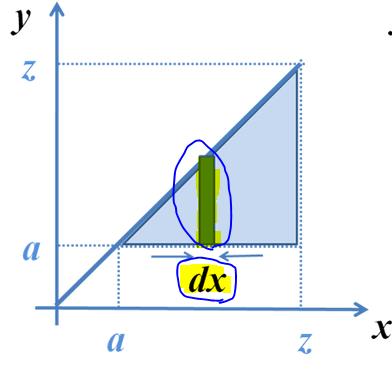
\includegraphics[width=0.8\textwidth]{Integration}
    \caption{Graphical Interpretation of the Differential}
    \label{figure:differential}
\end{figure}

To illustrate how we would be able to estimate the function itself using only the differential, imagine ascending differentials from the x-axis that `fit' this function. If our differential size was equal to $.1$, we would see that our first differential at $ x = .1 $ gives the value of $ y = .1 $. Our second at $ x = .2 $ gives a bar that is $.2$ units tall, our third at $ x = .3 $ gives a differential that is $.3$ units tall, and so on until we realize that the pattern is that the height of the differential is always the same value as $x$. From these observations, we are able to correctly induce that the function responsible for this layout of the differential is $ y = f(x) = x $. The process just described is essentially taking the integral of the function of $y$ at these various points of the differential. Integration, then, can be understood as summing these bars which represent the differential. Tolsoy is proposing a similar method by which the broad scheme of history, our function of $x$, can be known by integrating the differentials of history, which for him are the daily lives and particulars of each individual in his novel.

\pagebreak

\begingroup
\renewcommand{\section}[2]{}	% in article, this becomes reference, so we suppress the normal \section\refname
\centerline{\textbf{Bibliography}} 
\begin{thebibliography}{9}
\bibitem{tolstoy}
  Tolstoy, Leo. \emph{War and Peace: The Maude Translation, Backgrounds and Sources, Criticism.}
  Trans. Louise Maude and Aylmer Maude. Ed. George Gibian. New York: Norton, 1996. Print.
\end{thebibliography}

\endgroup

\end{document}
